\subsection{Solving data hazards}
\begin{figure}[!ht]
    \centering
    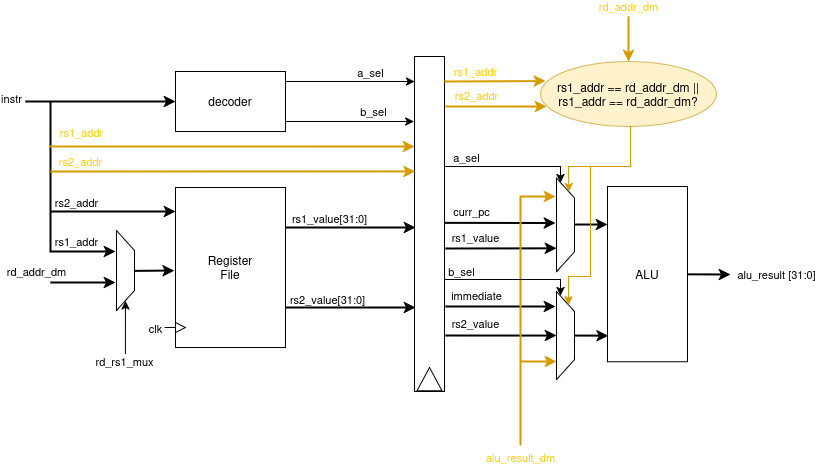
\includegraphics[scale = 0.3]{op_fw_datapath.png}
    \label{fig:op_fw}
    \caption{Concept for operand forwarding for solving data hazards}
\end{figure}

Pipelined architectures change the core system in order to execute instructions partially and with each segment being executed in sequence. This allows for faster clock and a higher throughput, but the fact that each instruction is initiated, in its execution, just a clock cycle later than the previous one introduces a crippling problem regarding the addressing of the same register in consecutive commands, as it happened in the previous simulation (Figure \ref{fig:DPPPL_sim}). This problem can be solved easily by either stalling the pipeline or by passing down the result of the ALU to another stage when needed, also called operand forwarding.
By comparing the destination register of the previous instructions, both in the DM and WB stages, and the operands of the next one, the datapath can be programmed to not increment the PC, thus stalling the pipeline for some clock cycles; Although simple, the solution is wasteful and can lead to slowdowns during very intensive arithmetic operations.
Operand Forwarding could instead have the execution flow just as before and still solve the problem; By adopting the same comparison method, the multiplexers at the ALU's inputs can select the previous result when necessary, and when the same register is addressed multiple times before it can be written, the most recent data can be used.\\
To successfully implement operand forwarding inside the IE, there is the need to analyze the previous destination register's address that has been passed down to both DM and WB, as said earlier, then confront both of the addresses with the address of each one of the operands and finally overwrite them with the most recent ALU's output. A VHDL description could be given below:

\begin{minted}[fontsize=\footnotesize]{vhdl}
    rs1_fw          <= alu_result_wb when (rd_addr_wb = rs1_addr_in) 
                        else alu_result_dm when (rd_addr_dm = rs1_addr_in)
                        else rs1_value_in;
    rs2_fw          <= alu_result_wb when (rd_addr_wb = rs2_addr_in)
                        else alu_result_dm when (rd_addr_dm = rs2_addr_in) 
                        else rs2_value_in;
    first_operand   <= rs1_fw when a_sel = '1' else curr_pc;
    second_operand  <= rs2_fw when b_sel = '1' else imm_se;
\end{minted}

However this code is incomplete, including the fact that the forwarded value for rs2 has to reach the data memory for the right value to be stored (which can already be dealt with by having \emph{rs2{\_}fw} as output from the IE), the register file will always be written after 3 clock cycles from the execution stage, meaning that there is another stage that must be covered, which is the ID. In this case an additional line can be added in order for the output of the register file to be overwritten if the register that has to be accessed has not been written yet:

\begin{minted}[fontsize=\footnotesize]{vhdl}
    reg : register_file
    port map(
        clk         => clk,
        da          => instr(11 downto 7) when op_class = "000110"  else 
                        instr(19 downto 15),
        pda         => instr(24 downto 20),
        dina        => rd_addr_in,
        din         => rd_value,
        we          => rd_write_en,
        rso         => rs1_value_reg,
        prso        => rs1_value_reg);

    rd_addr <= instr(11 downto 7);
    rs1_addr<= instr(19 downto 15);
    rs2_addr<= instr(24 downto 20);
    
    rs1_value_out <= rd_value when (instr(19 downto 15) = rd_addr_wb and rd_write_en = '1') 
                     else rs1_value_reg;
    rs2_value_out <= rd_value when (instr(24 downto 20) = rd_addr_wb and rd_write_en = '1') 
                     else rs1_value_reg;
\end{minted}
With the forwarding logic now ready, the simulation will show that the processor may be able to change the value of the operand with the latest data from other stages, this can be proven by having the store and load operation reading and writing from the same register as happens in the unpipelined datapath simulation.
In Figure \ref{fig:op_fw_sim} the withdrawed register values are shown in yellow, the forwarded values are highligted in orange. The final value used for each operand is shown in red and the results are exactly what expected, with the SW instruction having the ALU's result pointing at the address number 1, since the upper 19 bits of rs2 (containing 65540) are ignored (hence the resulting address should 4) with the first two bits as well, and with LW being able to address the same location in the memory, whose value is shown in the signal at the bottom to be in fact 131076.

\begin{figure}[!ht]
    \centering
    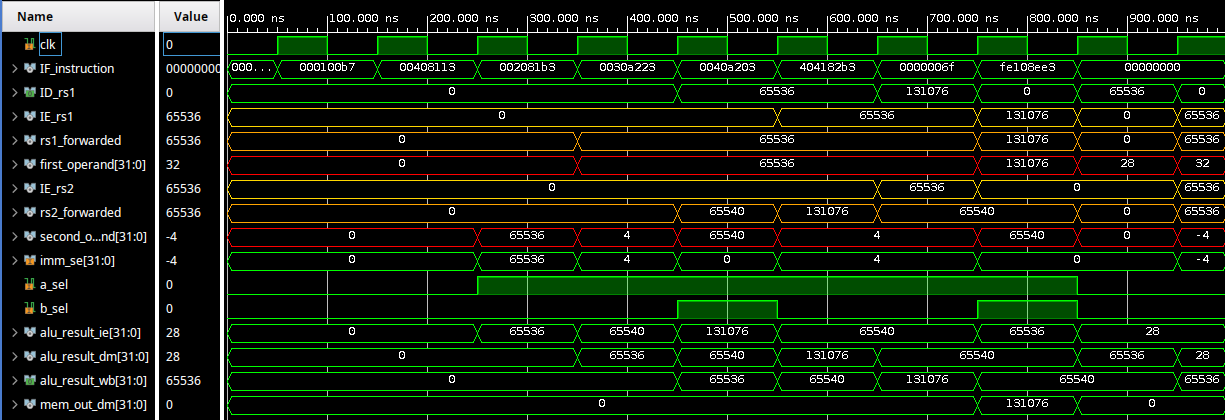
\includegraphics[scale = 0.35]{op_fw_sim.png}
    \label{fig:op_fw_sim}
    \caption{Datapath simulation with forwarding logic}
\end{figure}

\subsection{Managing control hazards}
